\documentclass[preprint]{aastex}
\usepackage{amsmath}
\usepackage{newtxtext, newtxmath}
\usepackage{booktabs}
\usepackage{graphicx}
\graphicspath{
  {../},
}
\usepackage{minted}

\usepackage{geometry}
\geometry{margin=1in}
\setkeys{Gin}{width=0.6\linewidth, keepaspectratio}  

\usepackage{natbib}
\usepackage{microtype}
\usepackage{xcolor}
\bibliographystyle{apj}

\newcommand\TsqDir{/Users/will/Work/RubinWFC3/Tsquared}
\input{\TsqDir/wfc3-macros.tex}


\begin{document}
\title{Orion fluctuations: New material 2015-10}
\author{W. J. Henney, C. R. O'Dell, G. J. Ferland, M. Peimbert}

\section{Temperature and density diagnostics from the MUSE data}
\label{sec:muse-diagnostic}


% 

\subsection{Maps at constant signal-to-noise}
\label{sec:maps-at-constant-snr}

\newcommand\MultibinFig[2]{\includegraphics{LineMaps/#1-multibin-SN#2}}



\subsection{Diagnostic plots}
\label{sec:diagnostic-plots}

\newcommand\DiagFig[3]{\includegraphics{muse-#1-#2-histogram-#3}}

\newcommand\siii{[\ion{S}{3}]}
\begin{figure}
  \setkeys{Gin}{width=0.45\linewidth}
  \begin{tabular}{ll}
    \MultibinFig{muse-derived-Te}{0003} 
    & \MultibinFig{muse-derived-Te-iii}{0003} \\
    \MultibinFig{muse-derived-Te}{0030} 
    & \MultibinFig{muse-derived-Te-iii}{0030} \\
    \MultibinFig{muse-derived-Te}{0300} 
    & \MultibinFig{muse-derived-Te-iii}{0300} \\
  \end{tabular}
  \caption{Temperature maps from MUSE spectra, adaptively binned to
    give constant signal-to-noise ratios of, top to bottom, 3, 30, and
    300. Left column \nii{} temperature, right column \siii{} temperature. }
  \label{fig:T-maps-snr}
\end{figure}

\begin{figure}
  \setkeys{Gin}{width=0.45\linewidth}
  \begin{tabular}{ll}
    \MultibinFig{muse-derived-Ne}{0003} 
    & \MultibinFig{muse-derived-Ne-iii}{0003} \\
    \MultibinFig{muse-derived-Ne}{0010} 
    & \MultibinFig{muse-derived-Ne-iii}{0010} \\
    \MultibinFig{muse-derived-Ne}{0030} 
    & \MultibinFig{muse-derived-Ne-iii}{0030} \\
  \end{tabular}
  \caption{Density maps at different signal-to-noise ratio. }
  \label{fig:T-maps-snr}
\end{figure}

\setlength\fboxsep{0.1\linewidth}
\newcommand\FourDiagsTest{%
  \framebox{A} &
  \framebox{B} &
  \framebox{C} &
  \framebox{D}
}
\newcommand\FourDiagsT[2]{%
  \DiagFig{log10_S_5755_}{T_N_II}{#1#2}&
  \DiagFig{log10_S_5755_}{N_II_Delta_T}{#1-fuzz000-bin#2}&
  \DiagFig{log10_S_6312_}{T_S_III}{#1#2}&
  \DiagFig{log10_S_6312_}{S_III_Delta_T}{#1-fuzz000-bin#2}
}
\newcommand\FourDiagsN[2]{%
  \DiagFig{log10_S_6716_}{log10_N_S_II_}{#1#2}&
  \DiagFig{log10_S_6716_}{S_II_log10-n}{#1-fuzz000-bin#2}&
  \DiagFig{log10_S_5518_}{log10_N_Cl_III_}{#1#2}&
  \DiagFig{log10_S_5518_}{Cl_III_log10-n}{#1-fuzz000-bin#2}
}
\newcommand\FourDiagsA[1]{%
  \DiagFig{log10_S_6716_}{log10_N_S_II_}{#1}&
  \DiagFig{log10_S_5518_}{log10_N_Cl_III_}{#1}&
  \DiagFig{log10_S_5755_}{T_N_II}{#1}&
  \DiagFig{log10_S_6312_}{T_S_III}{#1}
}
\newcommand\FourDiagsB[1]{%
  \DiagFig{log10_N_S_II_}{log10_N_Cl_III_}{#1}&
  \DiagFig{T_N_II}{T_S_III}{#1}&
  \DiagFig{log10_N_S_II_}{T_N_II}{#1}&
  \DiagFig{log10_N_Cl_III_}{T_S_III}{#1}
}
  
\newcommand\Binning[1]{%
  \raisebox{0.1\linewidth}{
    \shortstack{\(#1 \times #1\)\\ binning}
  }
}
\begin{figure}
  \setkeys{Gin}{width=0.2\linewidth}
  \footnotesize
  \begin{tabular}{r cccc}
    & \multicolumn{2}{c}{\dots {}[N II]{} Temperature \dots} &
    \multicolumn{2}{c}{\dots {}[S III]{} Temperature \dots} \\
    & Derived \(\Te\) & Noise estimate & Derived \(\Te\) & Noise estimate \\
    \Binning{1} & \FourDiagsT{full}{001}\\
    \Binning{4} & \FourDiagsT{full}{004}\\
    \Binning{16} & \FourDiagsT{full}{016}\\
    \Binning{64} & \FourDiagsT{full}{064}\\
  \end{tabular}
  \caption{Derived temperature versus surface brightness as a function of
    binning for the full MUSE field}
  \label{fig:muse-temp-diag}
\end{figure}

\begin{figure}
  \setkeys{Gin}{width=0.2\linewidth}
  \footnotesize
  \begin{tabular}{r cccc}
    & \multicolumn{2}{c}{\dots {}[S II]{} Density \dots} &
    \multicolumn{2}{c}{\dots {}[Cl III]{} Density \dots} \\
    & Derived \(\Ne\) & Noise estimate & Derived \(\Ne\) & Noise estimate \\
    \Binning{1} & \FourDiagsN{full}{001}\\
    \Binning{4} & \FourDiagsN{full}{004}\\
    \Binning{16} & \FourDiagsN{full}{016}\\
    \Binning{64} & \FourDiagsN{full}{064}\\
  \end{tabular}
  \caption{Derived density versus surface brightness as a function of
    binning for the full MUSE field}
  \label{fig:muse-density-diag}
\end{figure}


\newcommand\median{\ensuremath{\operatorname{median}}}
\begin{figure}
  \setkeys{Gin}{width=0.5\linewidth}
  \centering
  \begin{tabular}{@{}c@{}c@{}}
    Raw Values and Estimated Noise & Noise-Corrected Values \\ 
    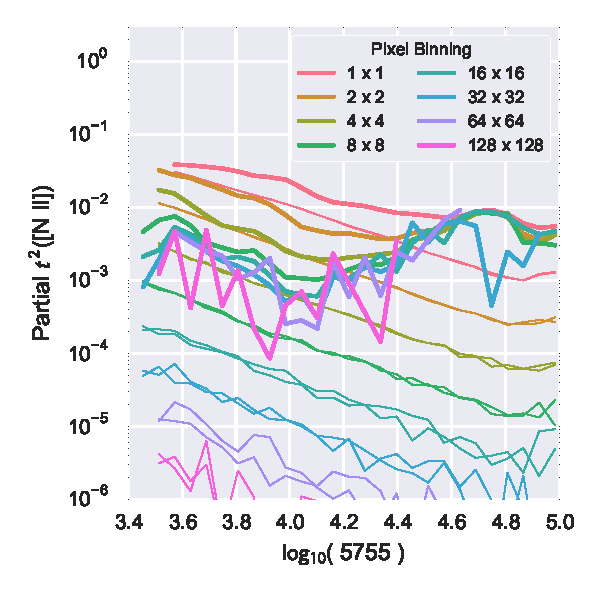
\includegraphics{muse-tsq-robust-vs-bright-N_II}
    & 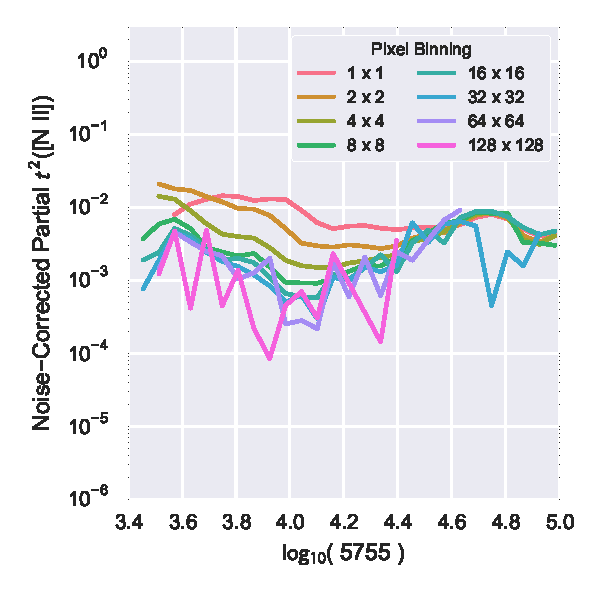
\includegraphics{muse-corrected-tsq-robust-vs-bright-N_II} \\
    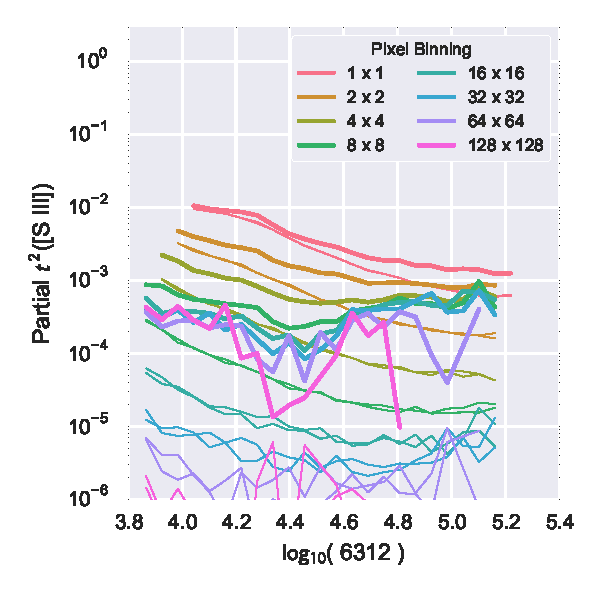
\includegraphics{muse-tsq-robust-vs-bright-S_III}
    & 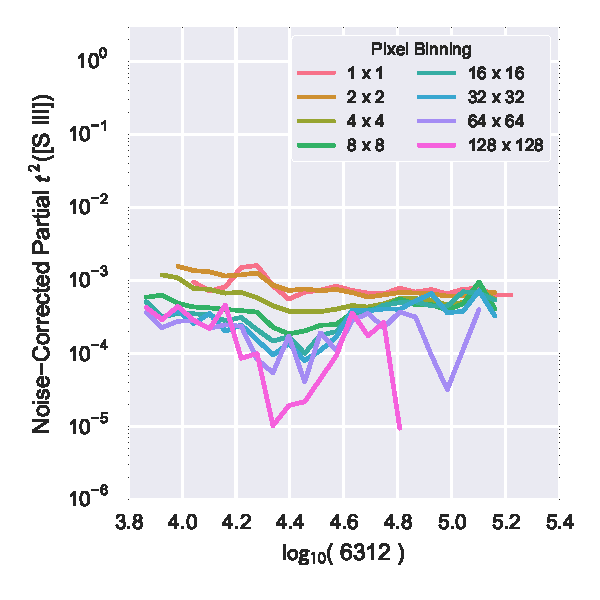
\includegraphics{muse-corrected-tsq-robust-vs-bright-S_III} \\
  \end{tabular}
  \caption{Partial \(t^2\) versus brightness for different pixel
    binnings.  In all cases \(t^2\) is calculated from a robust
    version of the variance: \(t^2 = \hat{\sigma}^2(T) / \median(T)^2\)
  \(\hat{\sigma} = 0.7413 \mathrm{IQR}\)}
  \label{fig:partial-t2}
\end{figure}


\begin{figure}
  \setkeys{Gin}{width=0.2\linewidth}
  \footnotesize
  \begin{tabular}{r cccc}
    & \multicolumn{2}{c}{\dots {}[N II]{} Temperature \dots} &
    \multicolumn{2}{c}{\dots {}[S III]{} Temperature \dots} \\
    & Derived \(\Te\) & Noise estimate & Derived \(\Te\) & Noise estimate \\
    \Binning{1} & \FourDiagsT{sweet}{001}\\
    \Binning{4} & \FourDiagsT{sweet}{004}\\
    \Binning{16} & \FourDiagsT{sweet}{016}\\
    \Binning{64} & \FourDiagsT{sweet}{064}\\
  \end{tabular}
  \caption{Derived temperature versus surface brightness as a function of
    binning for the MUSE data restricted to the WFC3 field.}
  \label{fig:muse-temp-diag-sweet}
\end{figure}

\begin{figure}
  \setkeys{Gin}{width=0.2\linewidth}
  \footnotesize
  \begin{tabular}{r cccc}
    & \multicolumn{2}{c}{\dots {}[S II]{} Density \dots} &
    \multicolumn{2}{c}{\dots {}[Cl III]{} Density \dots} \\
    & Derived \(\Ne\) & Noise estimate & Derived \(\Ne\) & Noise estimate \\
    \Binning{1} & \FourDiagsN{sweet}{001}\\
    \Binning{4} & \FourDiagsN{sweet}{004}\\
    \Binning{16} & \FourDiagsN{sweet}{016}\\
    \Binning{64} & \FourDiagsN{sweet}{064}\\
  \end{tabular}
  \caption{Derived density versus surface brightness as a function of
    binning for the MUSE data restricted to the WFC3 field.}
  \label{fig:muse-density-diag-sweet}
\end{figure}




\begin{figure}
  \setkeys{Gin}{width=0.2\linewidth}
  \footnotesize
  \begin{tabular}{l cccc}
    Binning & Density--Density & Temperature--Temperature & Density--Temperature & 
    Density--Temperature\\
    \raisebox{0.1\linewidth}{\(1 \times 1\)} & \FourDiagsB{full001}\\
    \raisebox{0.1\linewidth}{\(4 \times 4\)} & \FourDiagsB{full004}\\
    \raisebox{0.1\linewidth}{\(16 \times 16\)} & \FourDiagsB{full016}\\
    \raisebox{0.1\linewidth}{\(64 \times 64\)} & \FourDiagsB{full064}\\
  \end{tabular}
  \caption{Correlations between derived densities and temperatures as a function of
    binning for the full MUSE field}
  \label{fig:muse-dens-temp-correl}
\end{figure}

\begin{figure}
  \setkeys{Gin}{width=0.2\linewidth}
  \footnotesize
  \begin{tabular}{l cccc}
    Binning & Density--Density & Temperature--Temperature & Density--Temperature & 
    Density--Temperature\\
    \raisebox{0.1\linewidth}{\(1 \times 1\)} & \FourDiagsB{sweet001}\\
    \raisebox{0.1\linewidth}{\(4 \times 4\)} & \FourDiagsB{sweet004}\\
    \raisebox{0.1\linewidth}{\(16 \times 16\)} & \FourDiagsB{sweet016}\\
    \raisebox{0.1\linewidth}{\(64 \times 64\)} & \FourDiagsB{sweet064}\\
  \end{tabular}
  \caption{Correlations between derived densities and temperatures as a function of
    binning for the sweet spot.}
  \label{fig:muse-dens-temp-correl-sweet}
\end{figure}



\clearpage
\section{Absorption lines}
\label{sec:absorption-lines}

\begin{figure}
  \setkeys{Gin}{width=0.45\linewidth}
  \begin{tabular}{ll}
    (a) & (b) \\
    \MultibinFig{ew-N_III-6634}{0007} 
    & \MultibinFig{ew-He_II-4686}{0010} \\
    (c) & (d) \\
    \MultibinFig{ew-C_IV-5812}{0005} 
    & \MultibinFig{ew-N_III-5896}{0005} \\
  \end{tabular}
  \caption{Equivalent width of selected absorption lines from the MUSE
    spectra, adaptively binned to give constant signal-to-noise
    ratios. (\textit{a}) Mystery 6634 line. Traces absorption in
    PDR. (\textit{b}) \ion{He}{2} 4686 line.  Scattered starlight from \th2{A}
    (\textit{c}) \ion{C}{4} 5812 line. Scattered starlight from Trapezium.
    (\textit{d}) \ion{N}{3} 5896 line.  Scattered starlight, but filled
    in by fluorescent excitation in nebula?}
  \label{fig:T-maps-snr}
\end{figure}


\section{Fluorescent lines}
\label{sec:absorption-lines}

\begin{figure}
  \centering
  \setkeys{Gin}{width=\linewidth}
  \MultibinFig{ratio-7236-6563}{0030}
  \caption{Ratio of \ion{C}{2} 7236 to \ha}
  \label{fig:cii-halpha}
\end{figure}

\clearpage
\appendix
\section{New calibration of the WFC3 filters with MUSE}
\label{sec:muse-calib}
\citep{Weilbacher:2015a}


\newcommand\calibplot[1]{\includegraphics{wfc3-vs-muse-calib-#1}}

\begin{figure}[p]
  \centering
  \setkeys{Gin}{width=\linewidth}
  \calibplot{F656N}
  \caption[]{Results of spectrophotometric calibration of the WFC3 F656N
    filter.  The vertical axis of the principal plot is the observed
    WFC3 filter count rate after resampling at the \(0.2''\) pixel
    size of the MUSE spectrophotometric observations.  The horizontal
    axis of the principal plot is the predicted count rate calculated
    by folding the MUSE spectrum through the nominal WFC3 filter
    throughput profile.  The grayscale intensity represents the two-dimensional
    histogram over the entire usable WFC3 field of these two
    quantities, weighted by the count rate of each pixel.  The red
    line is the optimum linear fit to the relationship.  The lower
    right inset plot shows the product of the MUSE spectrum (integrated
    over the entire field) and the filter throughput profile.  The
    upper left inset plot shows the distribution of deviations from the
    linear fit for two subsamples of pixels: the red histogram shows
    the subsample with larger than average line/continuum ratio, while
    the blue histogram shows the subsample with smaller than average
    line/continuum ratio.}
\end{figure}

\newcommand\figcontinue[1]{
  \begin{figure}[p]
    \centering
    \setkeys{Gin}{width=\linewidth}
    \calibplot{#1}
    % \addtocounter{figure}{-1}
    \caption{#1}
  \end{figure}
}

\figcontinue{F658N}
\figcontinue{F502N}
\figcontinue{F673N}
\figcontinue{F487N}
\figcontinue{F469N}

\figcontinue{F547M}

\figcontinue{FQ575N}
\figcontinue{FQ672N}
\figcontinue{FQ674N}


\section{Comparison of spectrally derived and filter-derived line
  ratios}
\label{sec:comp-spectr-deriv}

\newcommand\ratioFig[2]{\includegraphics{NebulioMUSE/synthetic#1-vs-true-calib-#2}}

\newcommand\rowOfRatioFigs[1]{
  \ratioFig{-naive}{#1} & \ratioFig{-flat}{#1} & \ratioFig{}{#1} 
}
\begin{figure}
  \setkeys{Gin}{width=0.33\linewidth}
  \centering
  \begin{tabular}{lll}
    \rowOfRatioFigs{4861-6563} \\
    \rowOfRatioFigs{5755-6583} \\
    \rowOfRatioFigs{6716-6731} \\
    \rowOfRatioFigs{6716-6731-N} \\
  \end{tabular}
  \caption{Successive improvements in line ratio estimation using
    synthetic filters with the MUSE dataset}
\end{figure}


\clearpage

\bibliography{BibdeskLibrary-slavoj}


\end{document}
%%% Local Variables:
%%% mode: latex
%%% TeX-master: t
%%% End:


